
% ----- preamble -----
% {{{
\documentclass[journal=mamobx, layout=twocolumn]{achemso}

\usepackage{lipsum} % for generating dummy text
\usepackage[dvipsnames]{xcolor} % for colors
\usepackage{graphicx} % for figures
\usepackage{amsmath, amssymb} % for math
\usepackage{bm} % for bold math fonts
\usepackage{xr} % crossreferencing main manuscript to and from supporting info
\externaldocument[SI:]{suppinfo}
% }}}

% --- Title, Author Info, Abstract Text ---
% {{{
\title{How to Write a Research Paper}
\author{Douglas R. Tree}
\affiliation{Chemical Engineering Department, Brigham Young University, Provo, Utah}
\date{\today}
\email{tree.doug@byu.edu}

\newcommand*{\abstracttext}{
% Put abstract text here
This document provides instructions for making an \emph{outline} of a paper.
The instructions here correspond to Step $3$ of the process described in the README and in Whitesides article.
Once you have an outline (and data of course), writing a paper is a relatively straightforward (but often time-consuming) process.\\

\noindent\emph{At the outline stage, do not write an abstract.
Writing the abstract is typically the last step before you submit a paper.}
}

% for single column abstract
\let\oldmaketitle\maketitle
\let\maketitle\relax
% }}}

% ----- document text -----
\begin{document}

% Format the abstract (make one column, much better looking...)
% {{{
\twocolumn[
\begin{@twocolumnfalse}
  \oldmaketitle
  \begin{abstract}
    \abstracttext
  \end{abstract}
\end{@twocolumnfalse}
]
% }}}

\section{Introduction}
% {{{

Write out the first two or three paragraphs of an introduction.
Your introduction should be a ``funnel'' from the wider world into the research you are doing.
It should provide motivation and context for your paper.
It should also provide a ``scope'', i.e.\ what you are doing and what you are not trying to do, and it should provide a brief outline to orient the reader.

Specifically, your introduction should include the following pieces:
\begin{enumerate}
  \item Describe a ``problem'' and describe the state of the world that exists because of this problem
  \item Describe what others have done to solve this problem.
Focus on the ``prior state-of-the-art'', i.e.\ the best solution(s) that others have come up with, instead of a history lesson with all of the previous solutions.
You should have a few key references in this part~\cite{Tree2018}.
  \item Describe what your approach to solving the problem is. 
Focus on what is new or unique about your approach.
What are you doing that others haven't done before?
  \item Give a brief outline of how the paper is organized to orient the reader.
\end{enumerate}

% }}}

\section{Methods}
% {{{
\emph{Don't write a methods section at the outline stage.}
Usually a methods section is pretty easy to write when you get to the ``full paper'' stage.
You typically write down the details of what you did (as succinctly as possible) so that someone else can replicate your work.
The hard part is balancing details with brevity.
I will help you with this when the time comes.

% }}}

\section{Results and Discussion}
% {{{

Organize your results and discussion by subsections and figures.
Subsections are major organizing themes or topics for your figures.
Choose subsections that logically organize your results and tell a logical story.
Organize your figures within the subsections that does the same thing.

At the outline stage, do not write full paragraphs in the results and discussion.
However, you should put bulleted lists of what message you plan to convey along with each figure.
Every major point you want to discuss should have a figure, and every figure should be discussed.
If you are struggling to explain something, you probably need a figure, and you should never have figures that are disconnected from the text.

\subsection{How to add figures}

I have included an example figure, i.e.\ Fig~\ref{fig-placeholder} to show you how to do this in LaTeX, and how to do it in your outline.
You can reference a figure by its name in LaTeX; this makes it easy when you add or remove a figure.

\begin{figure}[tbp]
  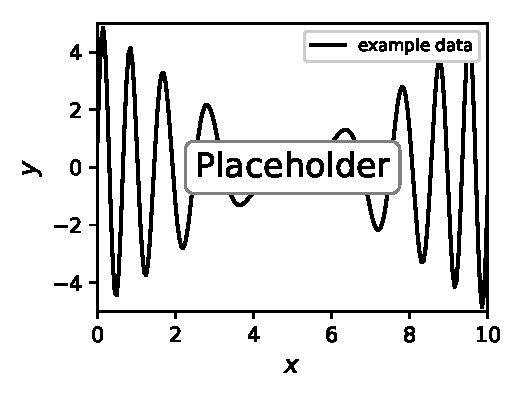
\includegraphics[width=3.25in]{fig-placeholder}
  \caption{This is a placeholder for the figure you should add. The caption should describe the figure and the necessary details.
It should not contain discussion of what the figure means.}
  \label{fig-placeholder}
\end{figure}

Your outline should include a list of points to make about your figure, e.g.\
\begin{itemize}
  \item How to add figures in LaTeX
  \item How to reference figures
  \item Adding bullet point lists in outlines
  \item Appropriate captions.
  \item Figure sizes
\end{itemize}

Note that most figures need to fit within a single column of a double column document.
The correct size in most journals is $3.25$ inches wide.
I like to make mine with an aspect ratio of $4\times3$, which gives a height of $2.44$ in, but you can choose an aspect ratio that you like.
If you need more space, you can make a double-wide figure of $6.5$ inches that spans two columns like Fig.~\ref{fig-doublewide}.
Keep the final figure size in mind while making your figures; it will save you a lot of time and effort in the end.
There are some example scripts in the \texttt{figure} directory that are hopefully useful to you.

\begin{figure*}[tbp]
  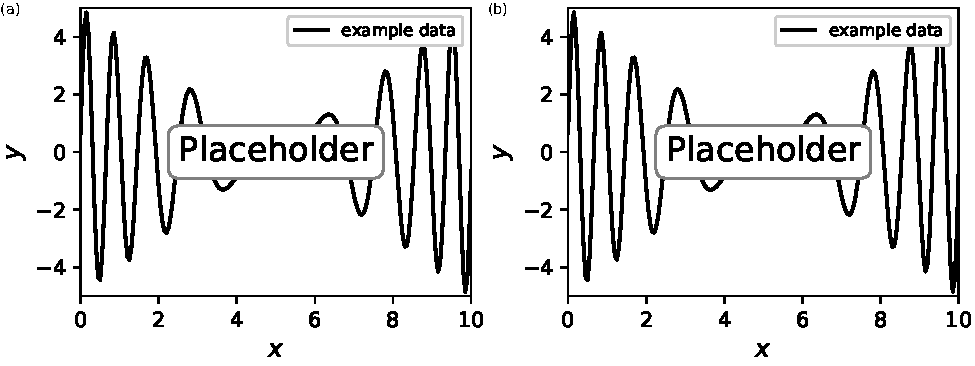
\includegraphics[width=6.5in]{fig-doublewide}
  \caption{This is a doublewide figure (spans both columns).}
  \label{fig-doublewide}
\end{figure*}

\subsection{How to add equations and tables}

You can add tables and equations to your paper as well as figures.
In the outline stage, you will probably have relatively few of these, but it is useful to see how to do this anyway.

Equations should be numbered, and should be inserted as part of a full sentence.
For example, the Pythagorean theorem
\begin{equation}
a^{2} = b^{2} + c^{2}
\end{equation}
could be an equation that you could include if you were going to write a paper on Fermat's last theorem.

Tables are inserted similarly to figures, as is shown by the example Table~\ref{tab-example}.
For more details, refer to the many online tutorials and examples of LaTeX tables.

\begin{table}
\caption{This is an example table}
\label{tab-example}
\begin{tabular}{cc}
\hline
Header 1 & Header 2 \\
\hline
R1, C1 & R1, C2 \\
R2, C1 & R2, C2 \\
\hline
\end{tabular}
\end{table}

% }}}

\section{Conclusion}
% {{{
Write a bulleted list here of the main conclusions of the paper.
These should include what the main, new contribution was to the problem outlined in the introduction.
The conclusion should be organized like an inverted funnel: start with the details of what you did and zoom out to state what the new state of the art is after you have completed your work.
The conclusion often terminates by stating what good ideas you have for future work.
% }}}

\begin{acknowledgement}
% {{{
% Acknowledgements of funding go here
We would like to acknowledge financial support from Brigham Young University and computational resources from the BYU Office of Research Computing.
% }}}
\end{acknowledgement}

\clearpage
\bibliography{refs}

\end{document}
